\documentclass[10pt]{article}
\usepackage[utf8]{inputenc}
\usepackage[russian]{babel}
\topmargin=-3cm
\textheight=24cm
\thispagestyle{empty}
\usepackage{graphicx}
\graphicspath{{/home/paul/Coding/Project/}}
\begin{document}
\begin{center}
{\bf \huge Software Development Plan: Распознавание цифр}
\end{center}
\section{Постановка задачи}
Перед авторами стоит задача создания программного продукта, функцией которого является распознавание рукописных цифр.
\section{Описание математической модели}
Написанная цифра, изначально представленная в виде изображения, рассматривается как вектор признаков, где признаки - пиксели данного изображения, а их значения - цвет пикселя (черный или белый). Данный вектор обрабатывается нейронной сетью, которая выдает прогноз, какой цифре соответствует тот или иной вектор.
\section{Постановка задачи на математической модели}
Исходя из предыдущего пункта, поставленная задача принимает следующий вид: требуется создать и обучить нейронную сеть, классифицирующую цифры с требуемой точностью.
\section{Алгоритмы и методы, используемые в модели}
Основная составляющая проекта - нейронная сеть, выделяющая характерные признаки полученного изображения и на их основе делающая прогноз. Реализуется на ЯП Python 2.7 с использованием библиотек Theano и Lasagne.


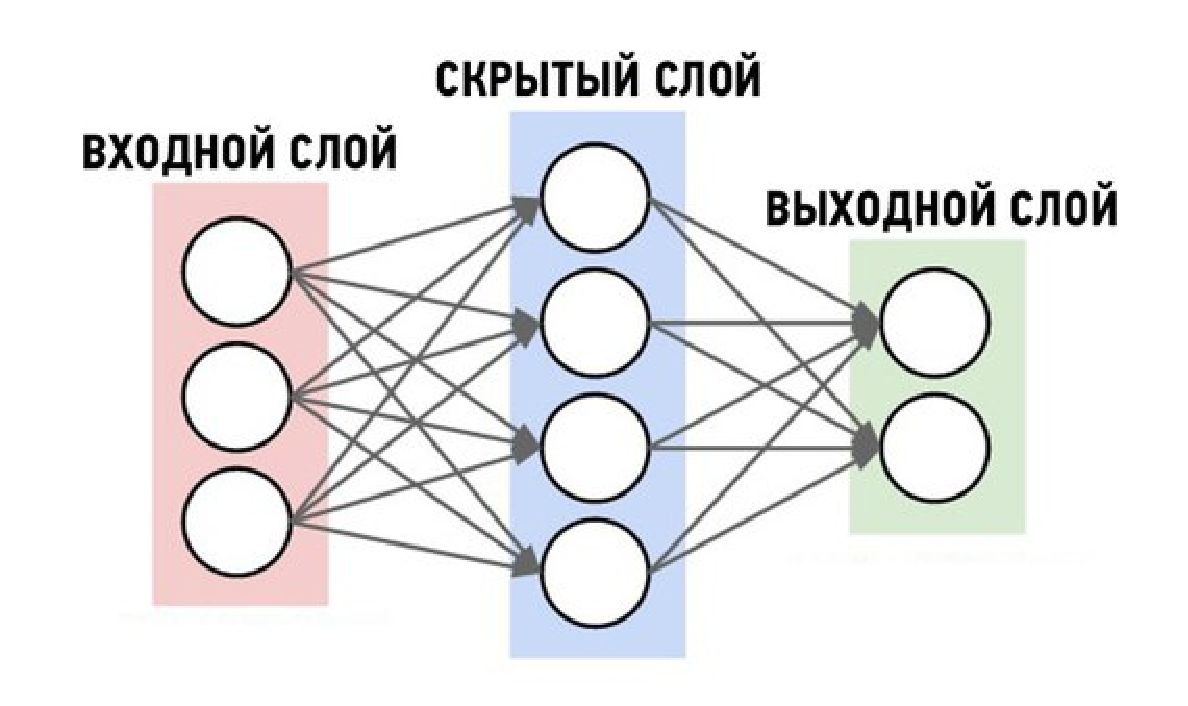
\includegraphics[width=0.5\linewidth]{Picture.eps}


Пользовательский интерфейс реализуется также на Python с использованием библиотек PyQt4 и Tkinter. В окне программы будет располагаться холст для рисования распознаваемой цифры, поле с результатом распознавания и уверенностью в прогнозе.
\section{Cписок участников и распределение задач}
\begin{enumerate}
\item Захаров Павел, 512 группа, ФРТК - графический интерфейс
\item Мокров Никита, 512 группа, ФРТК - нейронная сеть
\end{enumerate}
\end{document}